\chapter{Metasploit \cite{ivanbuetler}}
\newpage

\section{lecture}
\subsection{General Exploitation techniques}
\begin{itemize}
	\item Metasploit is a penetration testing framework and cybersecurity project that provides:
    \begin{itemize}
        \tightlist
		\item Tools for vulnerability identification
		\item A database of known exploits
		\item Payload development capabilities
		\item Post-exploitation modules
		\item Testing and verification tools
    \end{itemize}

	\item Key components:
    \begin{itemize}
        \tightlist
		\item Metasploit Framework (MSF) - The core open-source platform
		\item Meterpreter - Advanced payload for maintaining access
		\item Exploit modules - Pre-built attack code
		\item Auxiliary modules - For scanning and verification
		\item Post modules - For post-exploitation activities
    \end{itemize}

	\item Common uses:
    \begin{itemize}
        \tightlist
		\item Security testing by professionals
		\item Vulnerability validation
		\item Security research
		\item Network security assessments
		\item Testing defense systems
    \end{itemize}

	\item Key features:
    \begin{itemize}
        \tightlist
		\item Command line interface (msfconsole)
		\item Exploit development tools
		\item Payload generators
		\item Network discovery tools
		\item Automated exploitation capabilities
		\item Plugin architecture for extensibility
    \end{itemize}
\end{itemize}

It's important to note that while Metasploit is a legitimate security testing tool, it should only be used with proper authorization and in legal testing environments.

\subsection{Local exploit}
\begin{itemize}
	\item Executed directly on target system
	\item Requires existing access
	\item Exploits privilege escalation vulnerabilities
	\item Examples: Buffer overflows in local services, kernel exploits
  \subsubsection*{Metasploit context}
	\item Use 'local/' modules
	\item Post-exploitation phase
	\item Escalate privileges after initial access
	\item Example: \lstinline|windows/local/ms16_032_secondary_logon_handle_privesc|
\end{itemize}

\subsection{Server-side exploit}
\begin{itemize}
	\item Targets running services/applications
	\item Executed against remote systems
	\item Exploits network-facing services
	\item Examples: Web server vulnerabilities, database exploits
  \subsubsection*{Metasploit context}
	\item Use 'exploit/' modules
	\item Direct targeting of services
	\item Often uses specific ports
	\item Example: \lstinline|windows/smb/ms17_010_eternalblue|
\end{itemize}

\subsection{Client-side exploit}
\begin{itemize}
	\item Requires user interaction
	\item Targets client applications
	\item Relies on social engineering
	\item Examples: Malicious PDFs, browser exploits
  \subsubsection*{Metasploit context}
	\item Use 'exploit/windows/browser/' or similar
	\item Generate malicious files/content
	\item Often paired with social engineering
	\item Example: \lstinline|exploit/windows/fileformat/adobe_pdf_embedded_exe|
\end{itemize}


\subsection{Command \& Control (C2, C\&C)}
If we can execute arbitrary code on a remote host - what should we execute? Some sort of payload we can drop, so we can access the host later part of C\&C (Command \& Control)
\begin{itemize}
  \item Have some process or code which connects back to our server
  \item As user: have a fleet of hosts we can execute arbitrary code
\end{itemize}

\subsubsection*{Types of communcation}
\begin{itemize}
\item Shell Access:
  \begin{itemize}
    \tightlist
    \item Reverse shell (target connects back) \\ 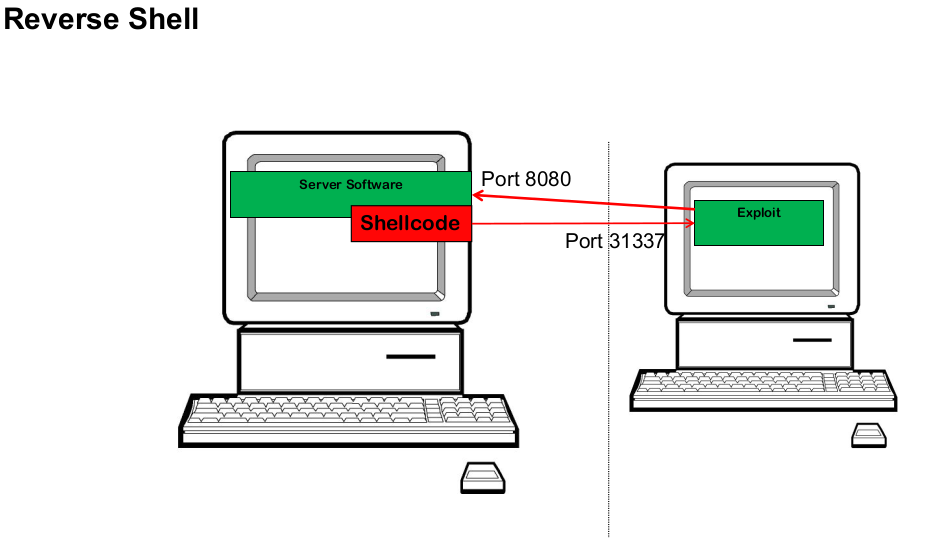
\includegraphics[scale=0.5]{resources/03-reverse-shell.png}
    \item Bind shell (connect to target) \\ 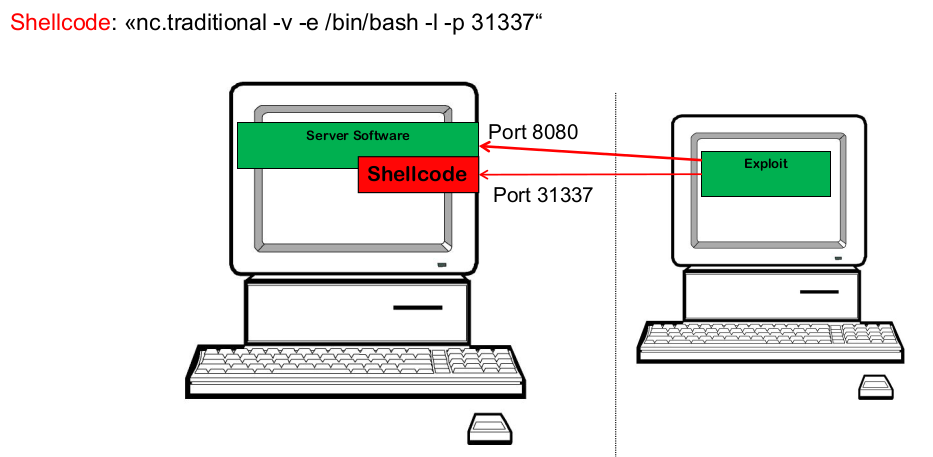
\includegraphics[scale=0.5]{resources/03-bind-shell.png}
    \item Web shell (via HTTP/HTTPS) \\ 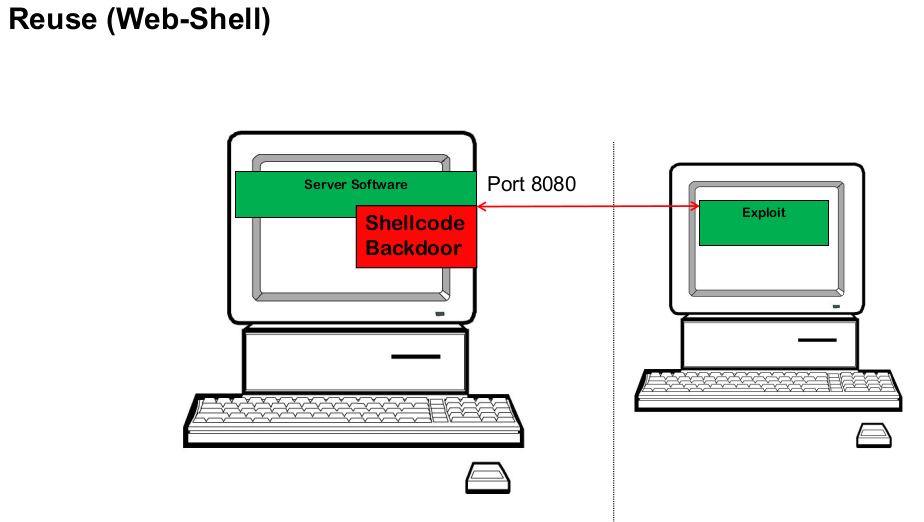
\includegraphics[scale=0.5]{resources/03-web-shell.png}
  \end{itemize}

\item Data Channel Types:
  \begin{itemize}
    \tightlist
    \item Direct HTTPS posts
    \item DNS tunneling
    \item ICMP tunneling
    \item WebSocket connections
    \item Proxy-aware communications
  \end{itemize}

\item Control Methods:
  \begin{itemize}
    \tightlist
    \item Real-time command execution
    \item Scheduled tasks
    \item Beacon responses
    \item Dead drop communications
    \item Multi-stage payloads
  \end{itemize}

\item Covert Channels:
  \begin{itemize}
  \tightlist
	\item Steganography
	\item Protocol tunneling
	\item Traffic mimicking
	\item Custom protocols
	\item Side-channel communications
  \end{itemize}
\end{itemize}
All these need to blend with normal traffic to avoid detection.

\subsection{Metasploit}
\begin{itemize}
\item Metasploit provides
  \begin{itemize}
    \tightlist
    \item Exploits
    \item Payloads
  \end{itemize}
  \item Payloads
  \begin{itemize}
    \tightlist
    \item (bash-) Shell
    \item Meterpreter
    \item "Meterpreter is an advanced, dynamically extensible payload that uses in-memory DLL injection stagers and is extended over the network at runtime. It communicates over the stager socket and provides a comprehensive client-side Ruby API. It features command history, tab completion, channels, and more."
  \end{itemize}
\end{itemize}

Metasploit supports all connection types
\begin{itemize}
  \item Bind-, Reverse-, Reuse-
  \item Can handle multiple connections (e.g. handle 20 exploited IE browser sessions)
  \item Meterpreter is stage-3 payload
  \begin{itemize}
    \tightlist
    \item Linux, Windows
    \item can execute commands
    \item Take screenshots
    \item load code
  \end{itemize}
\end{itemize}

\subsection{Metasploit Meterpreter}
\begin{itemize}
	\item Core Features:
  \begin{itemize}
    \tightlist
		\item In-memory execution (stealthy)
		\item DLL injection capabilities
		\item Extensible via modules
		\item Encrypted communication
  \end{itemize}

	\item Key Functionalities:
  \begin{itemize}
    \tightlist
		\item File system manipulation
		\item Process manipulation
		\item Registry interaction 
		\item Screenshot capture
		\item Keylogging
		\item Privilege escalation
		\item Network pivoting
  \end{itemize}

	\item Communication:
  \begin{itemize}
    \tightlist
		\item TLS encrypted channels
		\item Multiple transport protocols
		\item Staging capabilities
		\item Built-in port forwarding
		\item Proxy awareness
  \end{itemize}

	\item Advanced Features:
  \begin{itemize}
    \tightlist
		\item Migrate between processes
		\item Load additional modules dynamically
		\item Bypass AV through memory injection
		\item Multiple shell access types
		\item Python/PowerShell scripting integration
  \end{itemize}
\end{itemize}

\subsubsection*{Metasploit C2 Commands}
\begin{itemize}
	\item download\/upload: Transfer files between attacker and target system
  \begin{itemize}
    \tightlist
		\item download: Get files from target
		\item upload: Send files to target
	\end{itemize}

	\item edit: Open text editor to modify files on target

	\item execute: Run commands or programs on target system

	\item ipconfig: Display network configuration info (IP addresses, interfaces)

	\item shell: Drop into system command shell (cmd.exe or /bin/sh)

	\item hashdump: Extract Windows password hashes from SAM database for offline cracking

	\item migrate: Move Meterpreter to another process for persistence/stealth
  \begin{itemize}
    \tightlist
		\item Example: migrate from unstable to stable process
		\item Helps avoid detection
	\end{itemize}
	\item \lstinline|webcam_snap: Capture image from target's webcam if available|
\end{itemize}
These commands are core Meterpreter functions for post-exploitation activities after gaining access.

\subsection{Vulnerability Attacks}
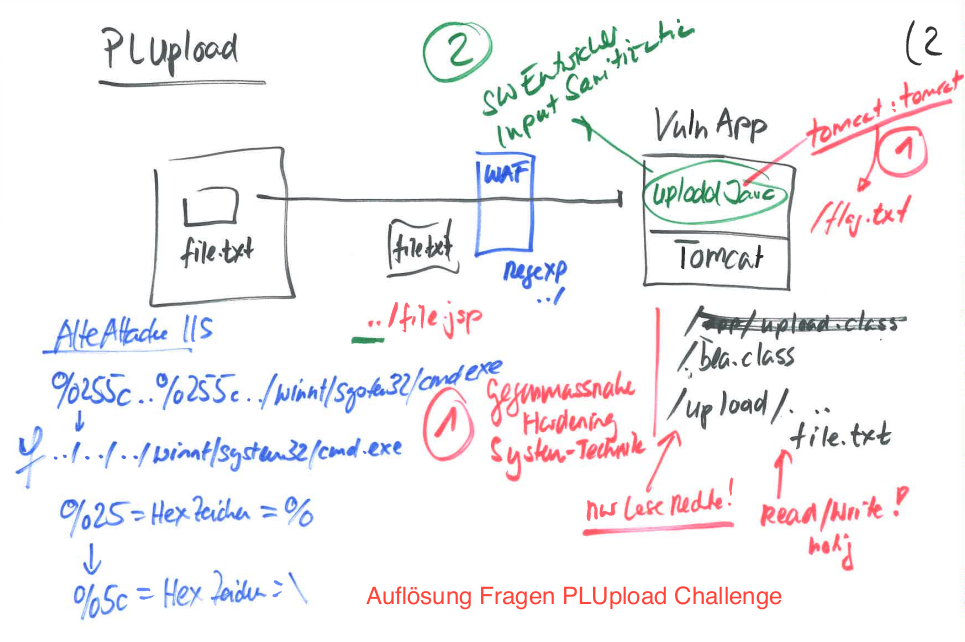
\includegraphics[scale=0.5]{resources/03-plupload.png}

\textbf{Diagram of fileupload vulnerability exploitation}
\begin{enumerate}
  \item File Upload Path:
  \begin{itemize}
    \tightlist
		\item File.txt being uploaded through WAF (Web Application Firewall)
		\item Tomcat server running a vulnerable upload application
  \end{itemize}

  \item Exploitation Method:
  \begin{itemize}
    \tightlist
		\item \lstinline|codeURL encoding/double encoding being used (%25 = hex for %, %5c = hex for \)|
		\item Directory traversal attempt using win/system32/cmd.exe
		\item Suggests trying to execute system commands via upload path
  \end{itemize}

  \item Attack Goals:
  \begin{itemize}
    \tightlist
		\item Bypassing input sanitization
		\item Achieving remote code execution through file upload
		\item Possibly exploiting path traversal vulnerability
  \end{itemize}
\end{enumerate}

This appears to be documentation for a "PLUpload Challenge" focused on exploiting file upload vulnerabilities in a web application.

For security reasons, I should note that this kind of knowledge should only be applied in authorized testing environments with proper permissions.

\textbf{Wifi Pineapple}
I'll explain WiFi Pineapple security risks and protections while staying within ethical bounds:

\begin{enumerate}
  \item Malicious Uses:
  \begin{itemize}
    \tightlist
		\item Man-in-the-middle attacks via rogue access points
		\item Network traffic interception 
		\item Credential harvesting
		\item Session hijacking
		\item Automated deauth attacks
  \end{itemize}

  \item Key Risks:
  \begin{itemize}
    \tightlist
		\item Public WiFi impersonation
		\item Evil twin attacks
		\item Transparent proxying
		\item SSL stripping
		\item Network mapping
  \end{itemize}
\end{enumerate}

Protection Measures:
\begin{enumerate}
  \item As a User:
  \begin{itemize}
    \tightlist
		\item Avoid public WiFi when possible
		\item Use VPN
		\item Enable HTTPS everywhere
		\item Verify network authenticity
		\item Check SSL certificates
  \end{itemize}

  \item As Organization:
  \begin{itemize}
    \tightlist
		\item Monitor for rogue APs
		\item Implement 802.1X
		\item Use strong WPA3 encryption
		\item Deploy wireless IDS/IPS
		\item Train users on WiFi security
  \end{itemize}
\end{enumerate}
Remember: Only use security tools like these in authorized testing environments with proper permissions.

\textbf{DNS tunneling}
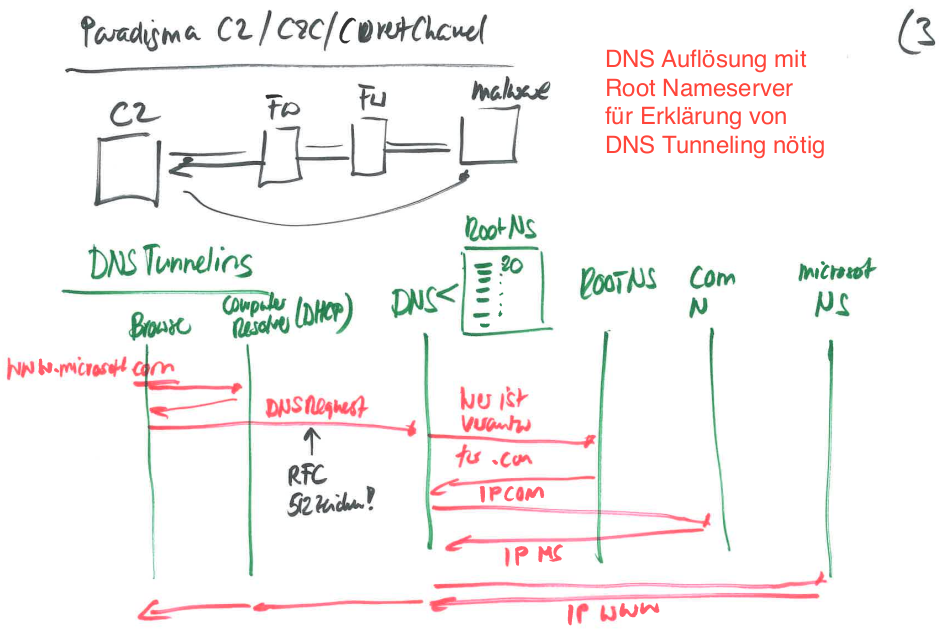
\includegraphics[scale=0.5]{resources/03-covert-channel.png}
\begin{enumerate}
  \item Architecture:
  \begin{itemize}
    \tightlist
		\item C2 server
		\item DNS tunneling through various channels (FW, FU, Malware)
		\item Root nameserver communication flow
  \end{itemize}

  \item DNS Resolution Process:
  \begin{itemize}
    \tightlist
		\item Browser initiates request to www.microsoft.com
		\item DNS request flows through hierarchy: Root NS → .com NS → Microsoft NS
		\item IPs returned through reverse path
  \end{itemize}
  \item "RFC 5C Ketten!" note suggests following RFC specifications for DNS chain/hierarchy
\end{enumerate}
This appears to be training material explaining DNS tunneling techniques, likely for security education purposes.

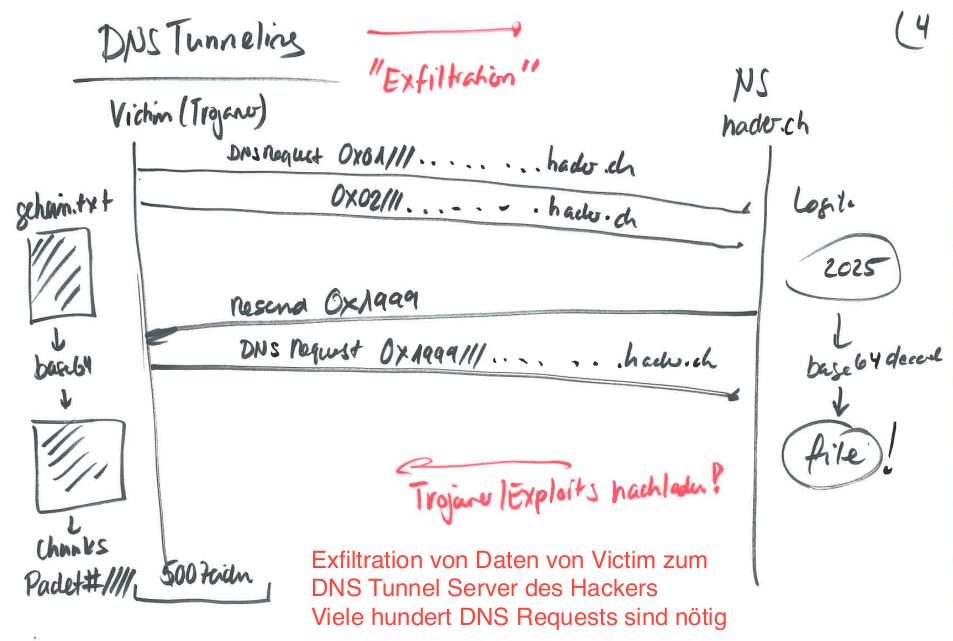
\includegraphics[scale=0.5]{resources/03-dns-tunneling-2.png}
\begin{enumerate}
  \item Process Flow:
  \begin{itemize}
    \tightlist
		\item Victim (with Trojan) chunks sensitive data (gehim.txt)
		\item Data encoded into DNS requests (0x0A///, 0x02///)
		\item Requests sent to hacker's DNS server (heder.ch)
		\item Server decodes base64 data into files
  \end{itemize}

  \item Key Elements:
  \begin{itemize}
    \tightlist
		\item 500KB data transmitted in chunks
		\item Multiple DNS requests required (noted as "Viele hundert" - many hundred)
		\item Hex-encoded data (0x4999///)
  \end{itemize}
\end{enumerate}
This illustrates how DNS tunneling can be used maliciously to steal data by encoding it within DNS queries, bypassing normal network controls.

\subsection{Secure architecture}

\textbf{Split DNS}
\begin{itemize}
	\item Architecture:
  \begin{itemize}
    \tightlist
		\item Internal DNS server (Firma) handles client requests
		\item DNS Firewall blocks direct FQDN resolution to internet
		\item Traffic routed through Proxy DNS and FW
  \end{itemize}

	\item Security Notes:
  \begin{itemize}
    \tightlist
		\item Blocks direct client-to-internet DNS resolution
		\item Companies use this to control DNS traffic
		\item Despite controls, data exfiltration still possible via web requests + DNS
  \end{itemize}
\end{itemize}
\begin{center}
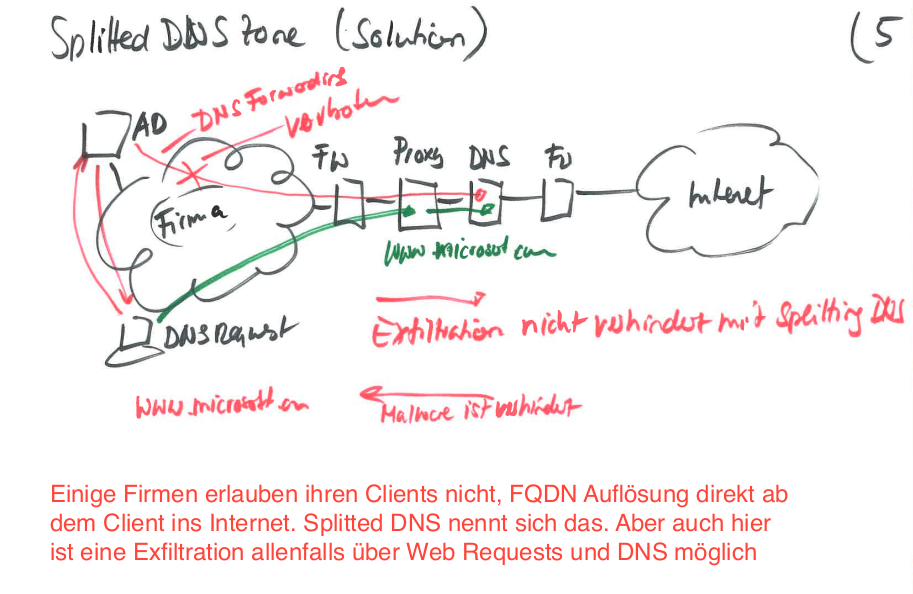
\includegraphics[width=\textwidth]{resources/03-split-dns.png}
\end{center}

This shows a defensive DNS architecture but highlights remaining exfiltration risks.

\textbf{DNS over HTTPS}
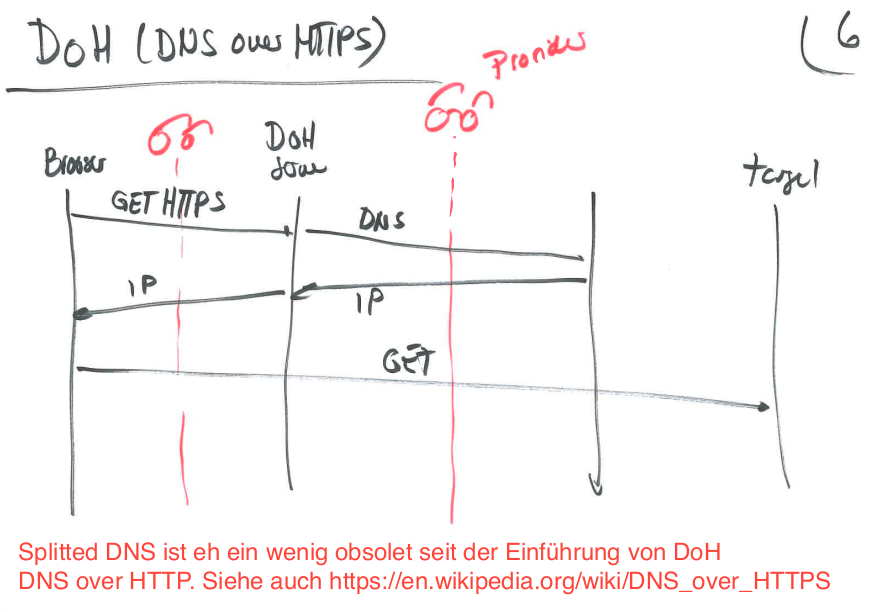
\includegraphics[width=\textwidth]{resources/03-dns-over-https.png}
DoH (DNS over HTTPS) encrypts DNS queries by sending them through HTTPS instead of plain UDP/TCP:

\begin{itemize}
  \item Purpose:
  \begin{itemize}
    \tightlist
		\item Privacy protection from ISPs/network observers
		\item Bypass DNS filtering/censorship
		\item Prevent DNS spoofing attacks
  \end{itemize}

  \item Circumvention methods; Network level:
  \begin{itemize}
    \tightlist
		\item Block known DoH providers
		\item Force traffic through local DNS
		\item Deep packet inspection
  \end{itemize}

	\item Enterprise:
  \begin{itemize}
    \tightlist
		\item Group policies to disable DoH
		\item Certificate controls
		\item Split DNS with strict egress filtering
  \end{itemize}
\end{itemize}

For security awareness: Organizations should have policies around DoH usage since it can bypass security controls, while also recognizing its legitimate privacy benefits.


\textbf{Proxy Request}
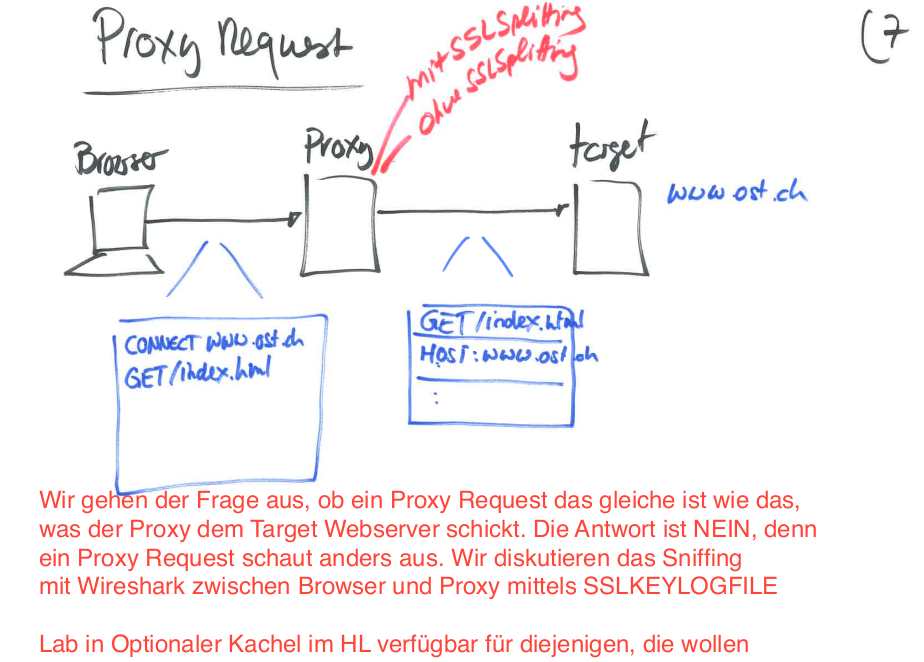
\includegraphics[scale=0.5]{resources/03-proxy-request.png}
Proxy servers act as intermediaries between clients and target servers:

\begin{itemize}
  \item Purpose:
  \begin{itemize}
    \tightlist
		\item Content filtering/monitoring
		\item Access control
		\item Traffic inspection
		\item Caching
		\item SSL/TLS inspection
  \end{itemize}

  \item Used for:
  \begin{itemize}
    \tightlist
		\item Enterprise security monitoring
		\item Content restrictions
		\item Performance optimization
		\item User activity logging
  \end{itemize}

  \item Circumvention methods; Technical:
  \begin{itemize}
    \tightlist
		\item VPNs/Tunneling
		\item Alternative ports
		\item Custom DNS
		\item Encrypted protocols
  \end{itemize}

	\item Detection avoidance:
  \begin{itemize}
    \tightlist
		\item Host file modifications
		\item Certificate pinning
		\item Direct IP connections
  \end{itemize}
\end{itemize}

Note: These techniques may violate organizational policies. Proxies often serve legitimate security purposes.
%
\section{exercise}